\documentclass[12pt,letterpaper]{report}
\usepackage[margin=1in]{geometry}
\usepackage{graphicx}
\usepackage{amsmath}
\usepackage[font=small,labelfont=bf]{caption}
\usepackage[justification=centering]{caption}
\usepackage{tikz}
\usepackage{circuitikz}
\usepackage{siunitx}
\usepackage{float}
\newlength \figwidth
\setlength \figwidth {0.75\linewidth}

\begin{document}

\title{E153 Laboratory Assignment \#7}
\author{Courtney Keeler and Stephen Pinto\\
Harvey Mudd College}
\date{November 20, 2013}
\maketitle

\section*{List of Materials}
\begin{itemize}
	\item Tektronix 2212 Oscilloscope
	\item Pomona 4550B (10X probe)
	\item Elenco LCM-1950 Multimeter
	\item 2N3904 transistor
	\item Standard resistors
	\item Standard capacitors
\end{itemize}

\section*{Purpose}
The purpose of this lab is to explore the Push Pull Amplifier by building one designed in class to compare with simulations, adding the Push Pull to the Common Emitter Amplifier from lab 6 to compare the results with the single emitter follower.

\section*{Push Pull Amplifier}

\begin{figure}[H]
\centering
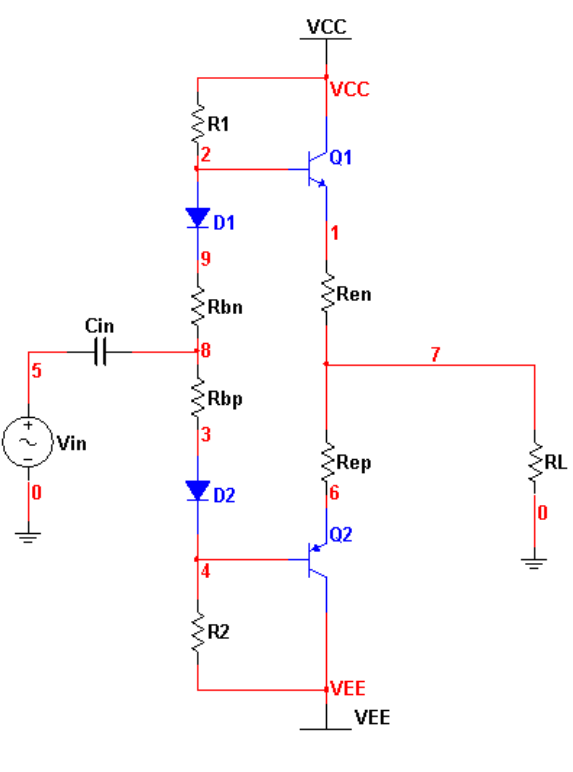
\includegraphics[width=\figwidth, keepaspectratio=true]{lab7_images/push_pull.png}
\caption{Class AB Push Pull Follower. Image from Lecture 12.}
\label{fig:push_pull}
\end{figure}

\subsection*{Procedure}

\begin{enumerate}
\item Measure the actual component values used in the Push Pull design (shown in Fig. \ref{fig:push_pull})
\item Build the Push Pull Amplifier with the measured components
\item Compare the actual gain and frequency response values with the simulated values
\end{enumerate}

\subsection*{Results}

Measured component values for the push pull follower:
\begin{itemize}
\item $R_1$ = 14.65 k$\Omega$
\item $R_{bn}$ = 15 $\Omega$
\item $R_{en}$ = 118 $\Omega$

\item $R_2$ = 14.76 k$\Omega$
\item $R_{bp}$ = 15 $\Omega$
\item $R_{ep}$ = 118 $\Omega$

\item $R_L$ = 981 $\Omega$
\end{itemize}


\subsection*{Calculations}


\subsection*{Analysis}


\section*{Conclusion}

In conclusion, this lab has shown that 
. The purposes of the lab, which was to build a pre-designed common emitter amplifier and compare the actual performance to the simulated performance, as well as  examine the effects of loading on the CE amplifier circuit, were met.

\end{document}

%photo 297: output of entire CE circuit, shows gain at 25 Hz
%photo 298: voltage after stage 1
%photo 299: voltage after emitter follower (it's been shifter down by 0.7!)

%\begin{table}[ht]
%\caption{Voltage across each "diode"} % title of Table
%\centering 
%    \begin{tabular}{| c | c |} 
%    \hline
%    $V_{\text{BC}}$ & 0.711 V \\
%    $V_{\text{BE}}$ & 0.717 V \\
%    \hline
%    \end{tabular}
%    \label{table:section_1}
%\end{table}

%input=500mvpp, 1kHz freq, high Z
%changing R1 of the CE amp to 15Mohm to try to lower the dc offset of output. new offset of output is 14.11 V (just within the +/- 5V requirement)
%output gain of CE: 4.741 V amplitude which means 10.22 Vpp (recall for 400 mV in)
%
%now we're changing R1 to 10K and R2 is 12K for now, may increase

%nevermind, we don't need to change the CE amp. We just have the consider the massive output impedance of the CE interfacing with the smaller input impedance of the push pull.
%
%photo 325: uncoupled output
%photo 326: coupled output (output from CE with a load)
%photo 327: DC offset CE amp output
%photo 328: push pull output (notice no DC offset!, but massive attenuation)

%npn beta is 183
